\chapter{Descripci\'on de la Metodologia}

WebML permite a los desarrolladores expresar los rasgos esenciales de un sitio 
de alto nivel. Los conceptos de WebML est\'an asociados a una representaci\'on 
gr\'afica e intuitiva, que puede ser apoyada por herramientas CASEs permiten una 
comunicaci\'on fluida entre dise\~nadores y programadores. La especificaci\'on de un
sitio con WebML se basa en la construcci\'on de modelos, estos son cuatro el
modelo estructural, el de hipertexto, el de presentaci\'on y el de 
personalizaci\'on, cada uno de ellos es esencial para obtener un buen 
resultado y no tener contratiempos en la etapa de codificaci\'on acontinuaci\'on se
brindar\'a una descripci\'on de cada uno de ellos.

\section{Modelo Estructural}

Expresa el contenido de los datos del sitio, no propone un nuevo lenguaje para 
el modelado de los datos ya que es compatible con el modelo de entidad relaci\'on 
y con los diagramas de clases propio de UML. Para hacer frente a la exigencia 
de presentar informaci\'on redundante y calculada, el modelo ofrece una 
simplificaci\'on, OQL (Object Query Language) como lenguaje de consulta, en la
que es posible especificar informaci\'on derivada. Este \'ultimo tambi\'en se lo
conoce como modelo de derivaci\'on. 

Por Ejemplo:

\begin{figure}[H]
    \centering
    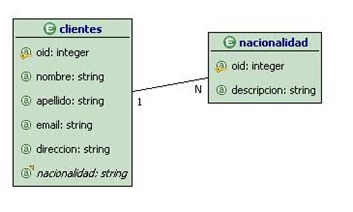
\includegraphics[scale=1]{resourse/extructura-esquema.jpg}
    \caption{Extructura de Esquema}
    \label{fig:01}
\end{figure}  

La Figura 1. muestra un esquema de estructura en el cual se muestran dos 
entidades relacionadas (diagrama realizado con la herramienta WebRatio), se
debe tener en cuenta que la herramienta utilizada modela la cardinalidad de la
relaci\'on al rev\'es de lo se acostumbra a ver, se debe leer as\'{\i} (muchos clientes
poseen la misma nacionalidad). Para hacer un ejemplo m\'as completo se decidi\'o
a\~nadir a la entidad clientes un atributo derivado nacionalidad: que mostrar\'{\i}a 
la nacionalidad de cada cliente. Esto sirve de ejemplo de modelo de derivaci\'on.


\section{Modelo de Hipertexto}

Describe uno o m\'as hipertextos que pueden ser publicados en el sitio. Cada 
hipertexto define un llamado sitio de vista, a su vez se divide en dos 
sub-modelos.


\subsection{Paginas}

Una p\'agina es una abstracci\'on de la regi\'on contenida en la pantalla, que es 
tratado como un bloque de interfaz independiente. Se puede ver como un 
contenedor de piezas de informaci\'on que se muestran al usuario, las cuales
pueden ser unidades u otras p\'aginas.

\begin{figure}[H]
    \centering
    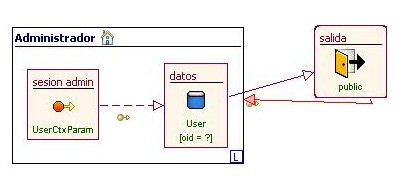
\includegraphics[scale=1]{resourse/salida-sitio-vista.jpg}
    \caption{Salida de un Sitio de vista}
    \label{fig:02}
\end{figure}  

La figura 2 muestra un ejemplo, se puede ver  unidades de contenido, la unidad
``datos" la cual muestra los datos de un usuario, tambi\'en podemos  ver algunas 
propiedades de la p\'agina por ejemplo el nombre: Administrador, el icono de
casita significa que es una p\'agina principal, etc. La tarea que realizan las
unidades que se encuentran descriptas en la tabla 1.

\subsection{Modelo de Composicion}

Especifica las p\'aginas que componen  el hipertexto, y el contenido de las 
unidades que componen la p\'agina. Se pueden utilizar siete tipos de unidades 
para componer las p\'aginas y estas son: Unidades de Datos, Datos m\'ultiples, 
\'{\i}ndice, el filtro, y el scroll. Las unidades de datos se utilizan para mostrar 
informaci\'on de un solo objeto (por ejemplo datos del personal), mientras que 
el resto de las unidades permite navegar de maneras alternativas por m\'ultiples 
objetos (por ejemplo todos los dict\'amenes que registro un usuario de personal).
A modo de aclaraci\'on la siguiente tabla muestra los tipos de unidades de
contenido que pueden ser usadas para componer una p\'agina: \\[0.5cm]

\begin{figure}[H]
    \centering
    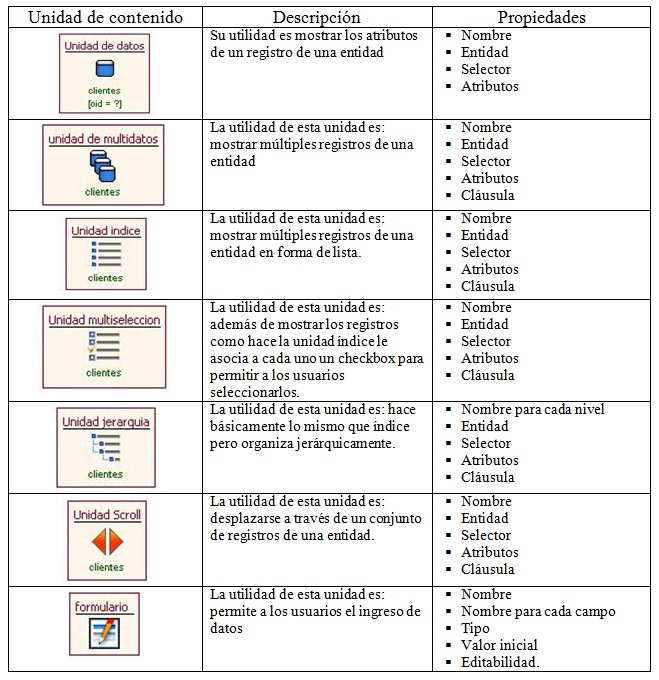
\includegraphics[scale=0.8]{resourse/tabla.jpg}
    \caption{Unidad de Contenido}
    \label{Tabla:01}
\end{figure} 

\footnote{ Los Iconos usados en la tabla fueron obtenidos de la Herramienta 
WebRatio}

\subsection{Modelo de Navegacion}

Expresa la forma y contenido de las p\'aginas que est\'an vinculadas a las 
unidades de forma de hipertexto. Los enlaces se pueden clasificar en dos ramas:

\begin{itemize}
    \item Los links contextuales: que acarrean justamente contenido o datos.
    De esta clase de links se puede hacer una subclasificaci\'on como: 
        \begin{enumerate}
            \item Links normales: son los que ve un usuario para hacer click y 
            navegar.   
            \item Links de transporte: solo ponen informaci\'on a disposici\'on 
            de la aplicaci\'on.    
        \end{enumerate}       
    \item Links no contextuales: son los que no acarrean ninguna tipo de valor
        o de informaci\'on para la p\'agina destino se dan entre p\'aginas 
        independientes
\end{itemize}        

Ejemplo: \\[0.5cm]

\begin{figure}[H]
    \centering
    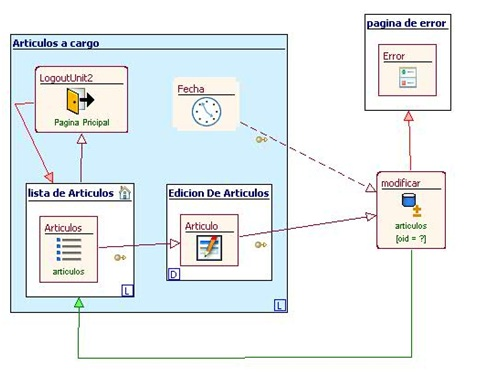
\includegraphics[scale=1]{resourse/modificar-articulo.jpg}
    \caption{Modificacion de Articulo}
    \label{TFig:03}
\end{figure} 

En la figura 3. Se puede apreciar un ejemplo un poco m\'as complejo que los 
anteriores pero no dif\'{\i}cil de entender. Se aprecian tres p\'aginas una p\'agina de
error, la segunda lista de Art\'{\i}culos que posee una unidad \'{\i}ndice, y por \'ultimo
la p\'agina Edici\'on de Art\'{\i}culos que posee un formulario, se puede apreciar que
entre estas dos \'ultimas hay un link, este link lleva la informaci\'on del 
articulo seleccionado al formulario para cargar los campos que ser\'aneditados
(link contextual), una vez editados se actualizar\'an en la base de datos a
trav\'es de la unidad modificar (v\'ease el otro link que va del formulario a la
unidad modificar). Hasta aqu\'{\i} s\'olo se vieron links contextuales normales, pero
hay otro el de l\'{\i}nea punteada que va desde fecha hasta la unidad modificar
(este es un link de transporte). Este se encarga de guardar la fecha de 
modificaci\'on del art\'{\i}culo y no se activa con un click. Ahora toca ver los
links no contextuales son los dos que salen de la unidad de la unidad modificar
(si hubo un error en la modificaci\'on se dirige a p\'agina de error y en caso
contrario vuelve a la p\'agina lista de art\'{\i}culos para editar otro si se desea).

\section{Modelo de Presentaci\'on}

Se refiere a la apariencia de las p\'aginas identificadas por el modelo de 
composici\'on. En WebML las p\'aginas se presentan de acuerdo a una hoja de estilo.
Una hoja de estilo dicta el dise\~no de p\'aginas y los elementos de contenido que 
se incluir\'a en dicha disposici\'on, y es independiente del lenguaje utilizado
para las p\'aginas a entregar. \\[0.5cm]

Para una mejor reutilizaci\'on, hay dos categor\'{\i}as de hojas de estilo y son:
\\[0.5cm]

\begin{itemize}
    \item Untyped: en estas hojas de estilo se describe el dise\~no de la 
        p\'agina independiente de su contenido, y, por tanto, puede aplicarse 
        independientemente de la cartograf\'{\i}a de la p\'agina a un determinado
        concepto.        
    \item Cartograf\'{\i}a: estas hojas de estilo son fijadas en una granularidad
        mas fina y, por lo tanto, s\'olo se aplican a p\'aginas que describen
        conceptos espec\'{\i}ficos o sea est\'an escritas para p\'aginas especificas.
\end{itemize}

\section{Modelo de Personalizaci\'on}

Los modelos de usuario y de grupos de usuarios est\'an expl\'{\i}citamente modelados en 
la estructura datos en forma de entidades predefinidas llamadas usuarios y
grupos, las caracter\'{\i}sticas de estas entidades se pueden utilizar para
almacenar un grupo espec\'{\i}fico de contenido. Este contenido personalizado
se puede utilizar tanto en la composici\'on de unidades o en la definici\'on de las 
especificaciones de presentaci\'on.  Adem\'as de puede representar aqu\'{\i} las reglas
del negocio. \\[0.5cm]

En sitios Web con p\'aginas de acceso p\'ublico y restringido, se pueden plantear
las siguientes cuestiones: \\[0.5cm]

\begin{itemize}
    \item Una o m\'as p\'aginas son accedidas por cualquier usuario.
    \item Un conjunto de p\'aginas privadas es accedida luego de un login, 
        estas contienen datos y servicios personales.
\end{itemize}

Por esta raz\'on es necesario pensar en la personalizaci\'on en funci\'on del tipo 
de p\'aginas a publicar (qu\'e usuarios deben acceder a qu\'e p\'agina) y  datos a
mostrar (que usuarios necesitan o pueden acceder a determinados datos).\\[0.5cm]

La personalizaci\'on tiene tres facetas: \\[0.5cm]

\begin{itemize}
    \item Control de acceso: operaciones de login y logout para el 
        reconocimiento de usuarios.       
    \item Asignaci\'on de vistas del sitio: dependiendo del grupo de usuario al 
        cual pertenezca dicho usuario, algunas vistas del sitio le ser\'an
        accesibles.        
    \item Personalizaci\'on de p\'aginas: dependiendo del usuario o grupo y del 
        contenido de la p\'agina.       
\end{itemize}

\subsection{Usuarios y Grupos}

Los usuarios y grupos de usuarios est\'an modelados expl\'{\i}citamente en el esquema
de estructura en la forma de entidades predefinidas llamadas usuarios y grupos.
Cada usuario puede pertenecer a uno o m\'as grupos, pero tiene un grupo 
predefinido para muchos usuarios, el esquema que se muestra en la figura 4
muestra la relaci\'on que existe entre usuarios y grupos. \\[0.5cm]

Tambi\'en se pueden declarar vistas del sitio especificando aspectos comunes de 
presentaci\'on teniendo en cuenta el tipo de usuario que posee el sitio, lo que
se trata de expresar es que cada grupo tiene un SiteView asociado tambi\'en se
puede observar esto en la figura 4.

\begin{figure}[H]
    \centering
    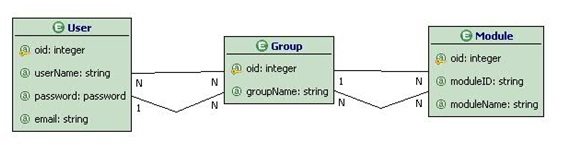
\includegraphics[scale=1]{resourse/usuarios.jpg}
    \caption{Entidades Involucradas}
    \label{TFig:04}
\end{figure} 


\subsection{Acceso Anonimo}

WebML posee un grupo predefinido llamado: ``Todos". Los usuarios que 
pertenecen a este, no necesitan registrarse para acceder ya que es un sitio 
p\'ublico (en WebRatio hacen dejando destildada la opci\'on ``protected" en el 
sitio de vista).

\subsection{LogIn y LogOut}

Una vista del sitio debe contener una p\'agina que permita a los usuarios 
loguears. La figura 5 muestra un diagrama asociado a un login (Iniciar Session
en el sistema) y la figura 6 muestra un logout (Cerrar Session).

\begin{figure}[H]
    \centering
    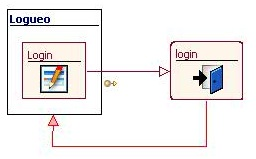
\includegraphics[scale=1]{resourse/login.jpg}
    \caption{Acceso de usuario a Sitio Protegido}
    \label{TFig:05}
\end{figure} 


En la figura 5. Se observa un formulario en la pagina Logueo (Login),
este posee dos campos usuario y contrase\~na. El v\'{\i}nculo que va a la unidad 
login lleva estos datos all\'{\i} de acuerdo a lo que indiquen las entidades 
usuario y grupo lo dirigir\'a a su respectivo sitio de vista.

\begin{figure}[H]
    \centering
    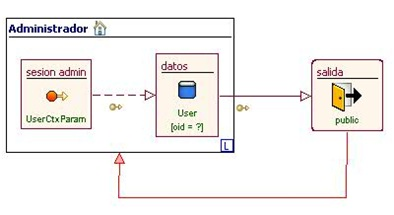
\includegraphics[scale=1]{resourse/logout.jpg}
    \caption{Salida de un sitio Protegido}
    \label{TFig:06}
\end{figure} 

En la Figura 6. Se puede apreciar que desde la unidad datos hay un v\'{\i}nculo a 
una unidad Logout (salida) de esta manera se abandona la vista de usuario 
(en este caso la del administrador). Se debe especificar a que vista se 
trasladar\'a el usuario en la unidad salida.


